\section{Thermodynamics}

\begin{center}
    Notes from \textbf{MECHENG 235: Thermodynamics I}

    Taken at University of Michigan, Fall 2024

    using \textit{Thermodynamics: an Engineering Approach}, by Boles and Cengel
\end{center}

\subsection{Basic Concepts of Thermodynamics}

\textbf{Thermodynamics} is the study of energy and its interaction with matter. In particular, \textit{classical thermodynamics} is the study of energy and energy transfer at a macroscopic level. Thermodynamics is concerned with the \textbf{equilibrium states} of systems.

A system has properties which may be \textbf{extensive} (varying with system size, i.e. total volume and total momentum) or \textbf{intensive} (not variable with size, i.e. temperature and pressure). A system is in \textit{equilibrium} when there are no forces driving change to the system. This equilibrium may be \textit{thermal} (temperature is constant with time), \textit{mechanical} (pressure is constant with time), or \textit{chemical} (chemical composition does not progress with time, no net reaction). A system may be \textbf{closed}, with a control mass and potentially variable volume, or \textbf{open}, with a control volume and potentially variable mass. A system is \textbf{adiabatic} if no heat is transferred (i.e. the system is well-insulated, or system is the same temperature as surroundings).

\begin{shaded}
    \textbf{The State Postulate.} The state of a simple compressible system is completely specified by \textit{two independent intensive properties}.
\end{shaded}

Other intensive properties of a system include \textbf{internal energy} $u$, and \textbf{enthalpy} $h$. Enthalpy is defined in terms of internal energy: \[H = U + PV\hspace{0.5in}(kJ)\] and specific enthalpy is similarly defined by \[h = u + Pv\hspace{0.5in}(kJ/kg)\] Internal energy is usually used in evaluating closed systems, while enthalpy may be used in evaluating open (flowing) systems.

\begin{shaded}
    \textbf{Zeroth Law of Thermodynamics.} If two bodies are in thermal equilibrium with a third body, they are also in thermal equilibrium with each other. If the third body is a thermometer, then the two bodies are in thermal equilibrium if they have the same temperature.
\end{shaded}

\subsection{Energy and the First Law of Thermodynamics}

Energy exists in several forms. There is \textbf{macroscopic energy} (kinetic, potential), \textbf{microscopic energy} (related to molecular structure and activity) and \textbf{internal energy, $U$} (sum of microscopic energies). In general, energy exists in either \textbf{static} or \textbf{dynamic} form:
\begin{enumerate}
    \item \textbf{Static energy}: stored in the system (ex. energy in chemical bonds).
    \item \textbf{Dynamic energy}: recognized only as it crosses a boundary (ex. heat, the flow of energy due to temperature difference at the boundaries; work, force applied to move a boundary)
\end{enumerate}

The \textbf{First Law of Thermodynamics} is the conservation law for energy:

\begin{shaded}
    \textbf{First Law of Thermodynamics.} Energy is not created or destroyed during a process and may only change forms. \[\underbrace{E_{in} - E_{out}}_{\text{macroscopic}} = \underbrace{\Delta E_{system}}_{\text{microscopic}}.\]
    For a cycle ($\Delta E_{system} = 0)$, the first law reduces to \[Q_{net}-W_{net} = 0\]
\end{shaded}

\subsection{Properties of Pure Substances}

A \textbf{pure substance} is any substance with a fixed, uniform chemical composition. A pure substance may be comprised of one element (i.e. nitrogen gas) or more (i.e. water), or a mixture of several substances which is homogeneous (i.e. air). The \textbf{phase} of a substance is dependent on the average movement of its molecules (temperature). During a \textbf{phase change}, some portion of a sample of substance exists in either phase, depending on the properties of substance. 

During a phase change from the liquid state to the gaseous state, a pure substance may be in any of the following phases:
\begin{enumerate}
    \item \textbf{Compressed liquid}. The substance is a liquid which is not about to vaporize.
    \item \textbf{Saturated liquid}. The substance is liquid, but any increase in temperature or decrease in pressure will cause it to partially vaporize.
    \item \textbf{Saturated liquid-vapor mixture}. The substance is a mix of gas and liquid. Without change to pressure, the temperature of a saturated vapor is constant, with only the volume changing during the process.
    \item \textbf{Saturated vapor}. The substance is a gas, but any decrease in temperature or increase in pressure will cause it to partially condense.
    \item \textbf{Superheated vapor}. The substance is a gas which is not about to vaporize.
\end{enumerate}

Pressure and temperature are dependent on each other during phase change, so another intensive property (generally specific volume, $v$) is required to describe the system. Plotting temperature or pressure against specific volume during a phase change gives the following:

\begin{center}
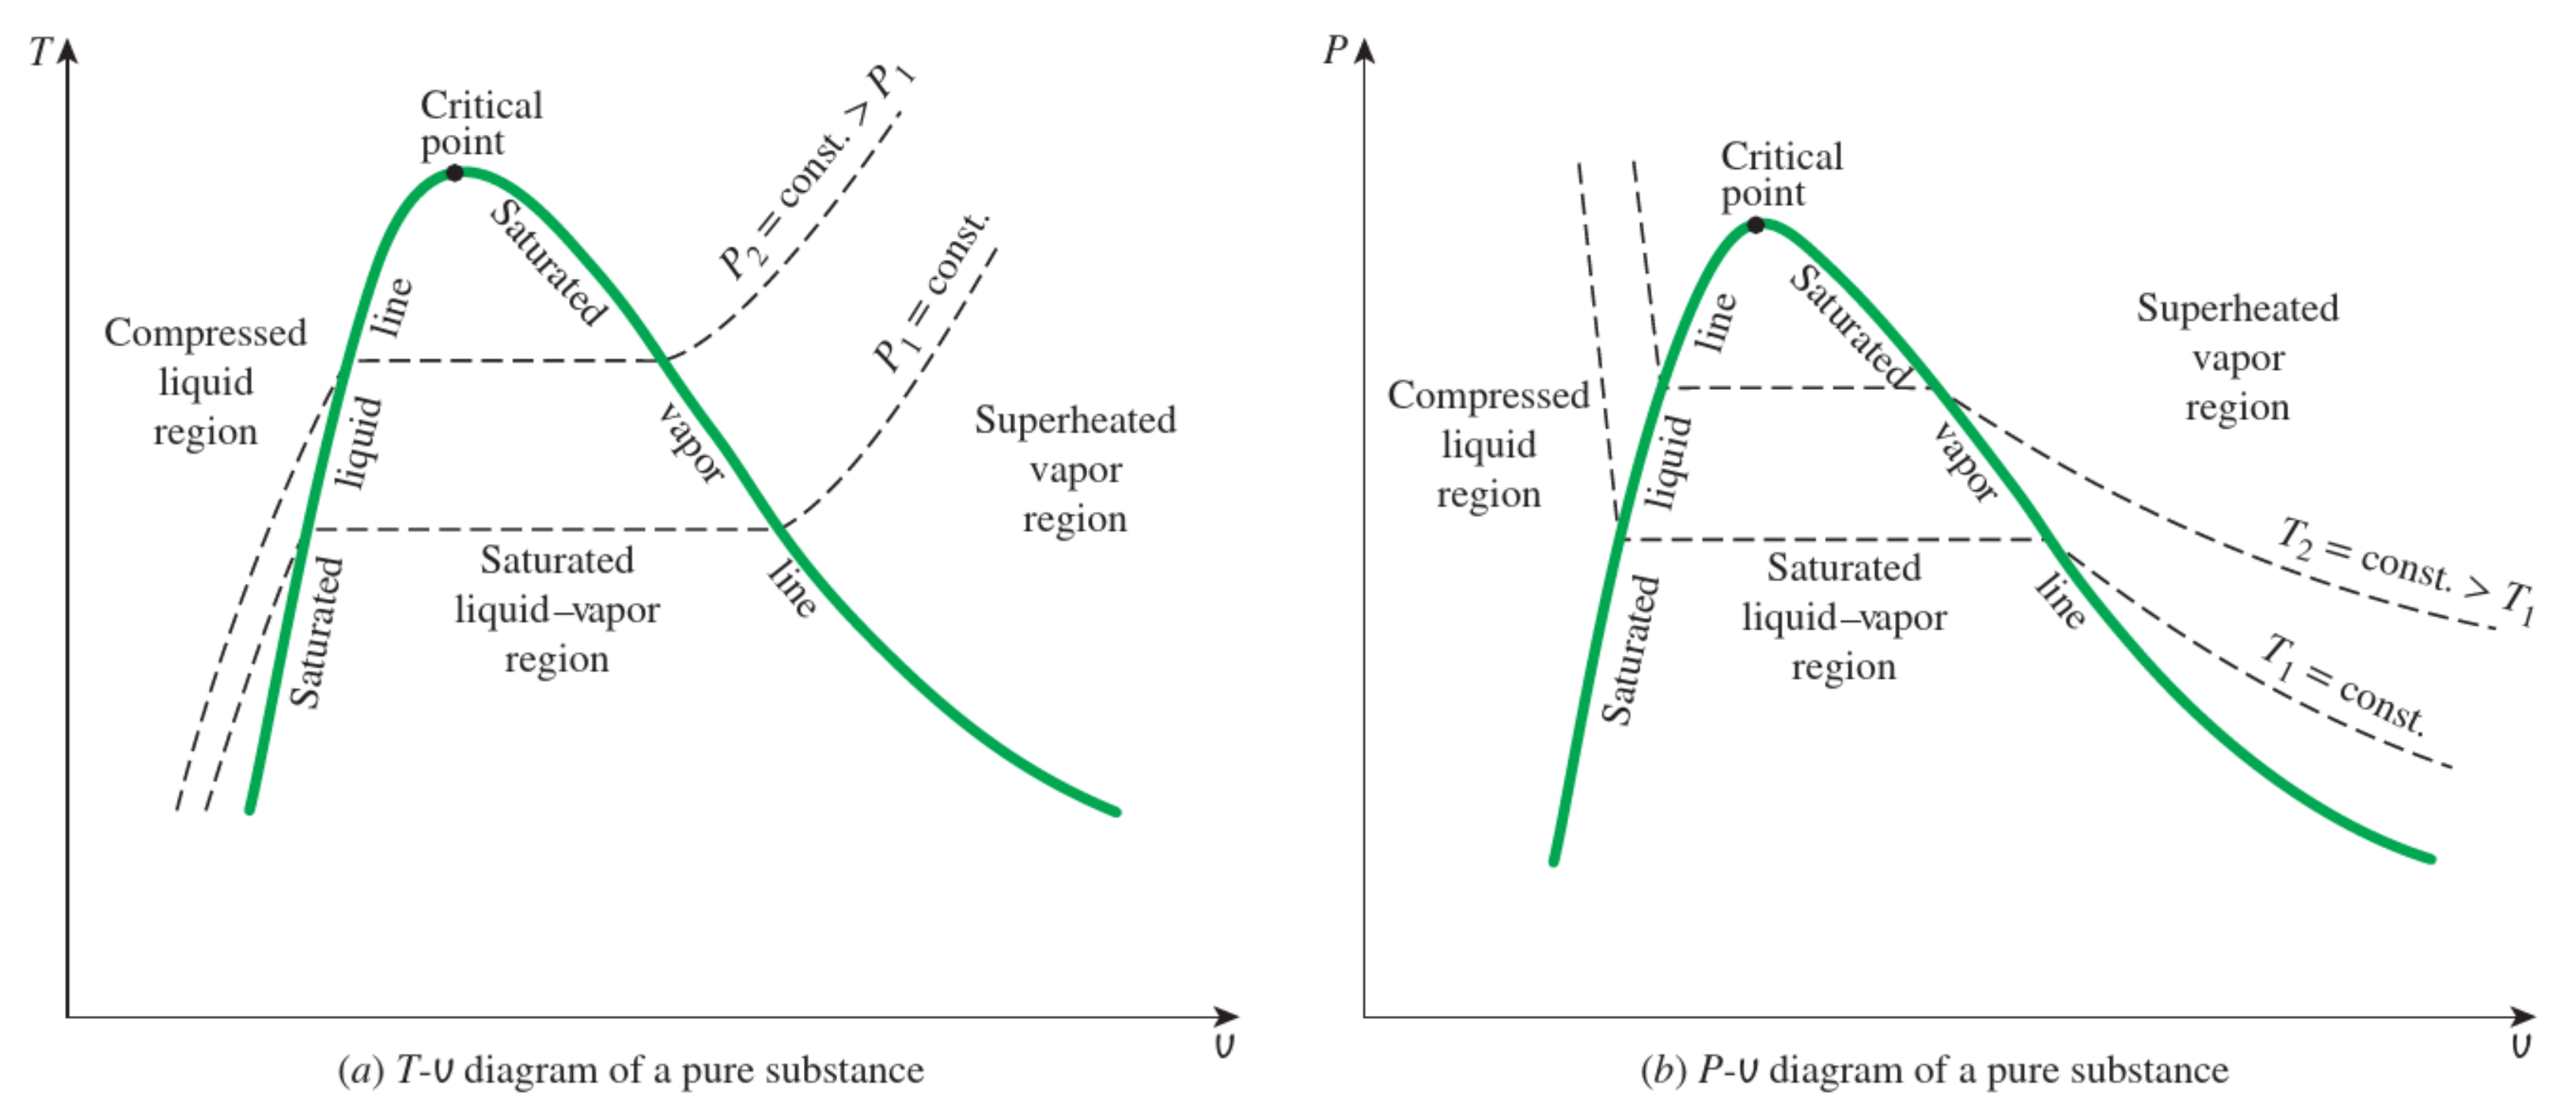
\includegraphics[width=\textwidth]{Images/thermo1.png}
\end{center}

The isolines show constant pressures or temperatures respectively. Importantly, holding pressure or temperature constant under the dome necessarily holds the other quantity constant.

%\newpage

\begin{shaded}
In general, an intensive property $p$ (standing in for volume, enthalpy, internal energy, etc) of a system are related to pressure and temperature by:
\begin{itemize}
    \item[] \textbf{Compressed liquid}: $p\approx p_{f}$ at $T$. Properties of a liquid at fixed temperature vary negligibly.
    \item[] \textbf{Saturated liquid}: $p=p_f$ from a property table.
    \item[] \textbf{Liquid-vapor mixture}: $p=p_f + x(v_g-v_f)$, where $x$ is the \textbf{quality} of the mixture, defined by the mass ratio of vapor to total mass: \[x=\frac{m_{\text{vapor}}}{m_\text{liquid}+m_\text{vapor}}\] Quality directly corresponds to a position along the horizontal portion of an isoline under the dome.
    \item[] \textbf{Saturated vapor}: $p=p_g$ from a property table.
    \item[] \textbf{Superheated vapor}: read from a property table for most values.
\end{itemize}
\end{shaded}

In absence of property tables, the \textbf{ideal gas law} sometimes provides a decent approximation for the behavior of gases. In particular, the ideal gas law is given by the equivalent relationships \[Pv=RT\hspace{0.325in}\text{or}\hspace{0.325in}PV=mRT\hspace{0.325in}\text{or}\hspace{0.325in}PV=nR_uT\] where $R$ is the gas constant for a specific substance and $R_u$ is the universal gas constant. Under certain conditions, a gas deviates from ideal behaviors. In this case, a \textbf{compressibility factor} $Z=v_\text{real}/v_\text{ideal}$ adjusts the ideal gas law: \[Pv=ZRT\] $Z$ is generally read from a compressibility chart (where $P_\text{cr}$ and $T_\text{cr}$ are particular to a substance and read from a table):
\begin{center}
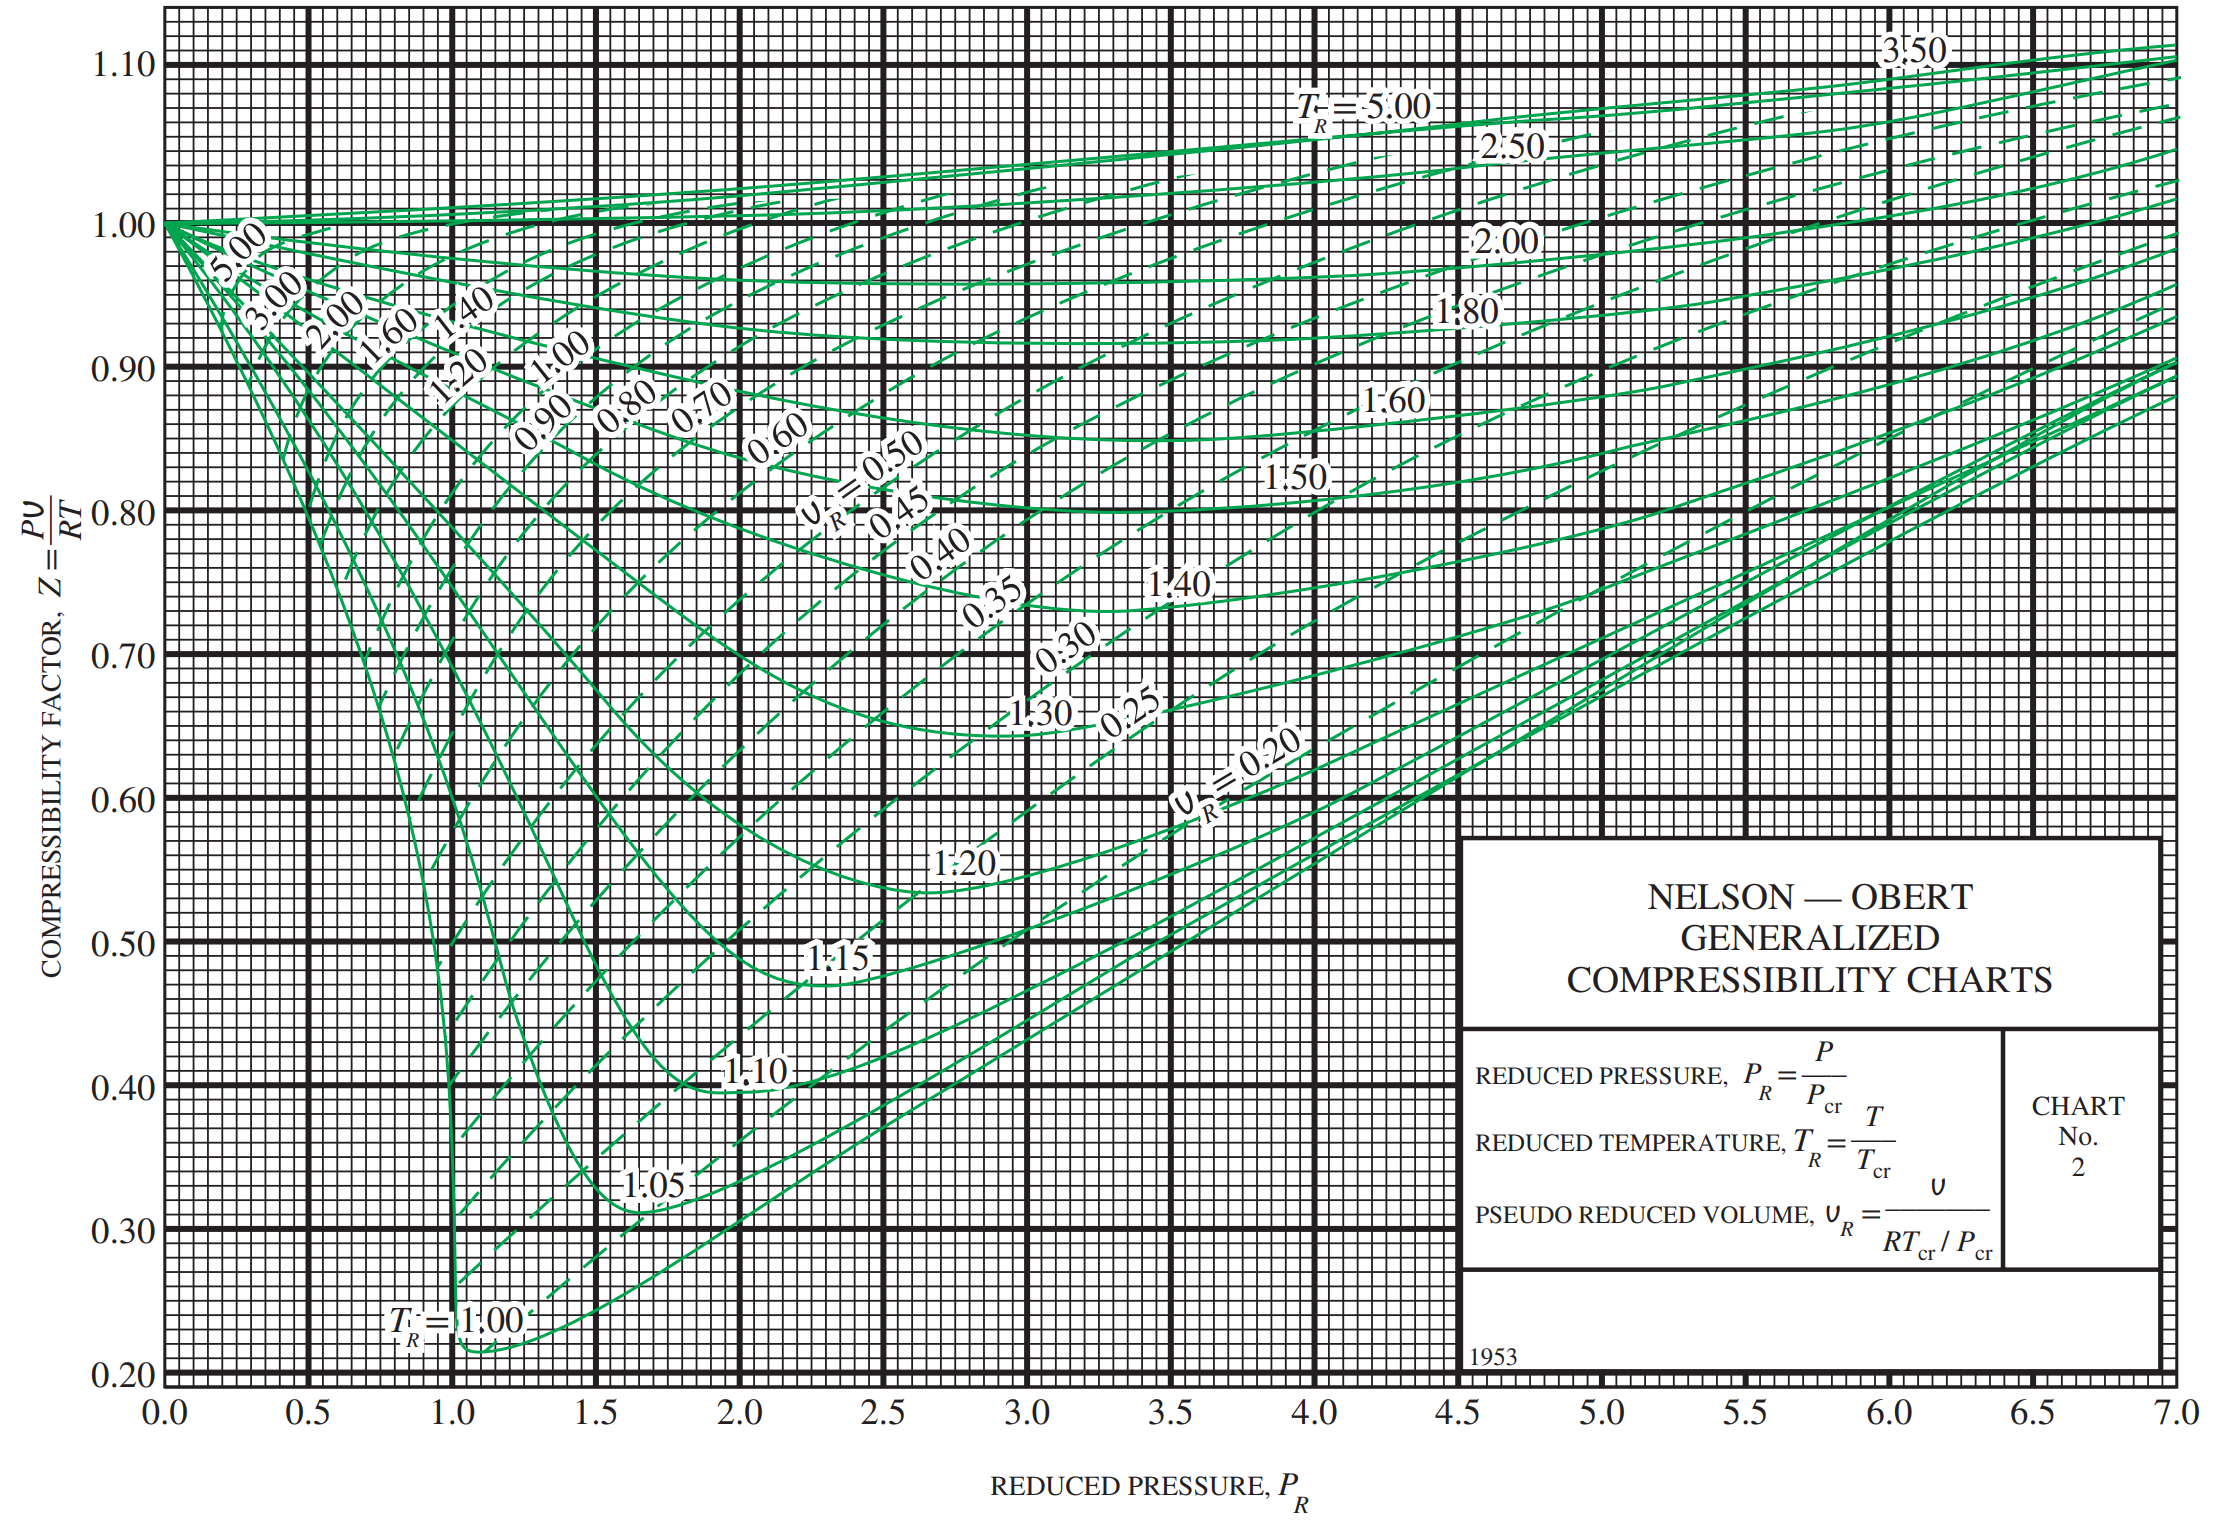
\includegraphics[width=0.85\linewidth]{Images/thermo2.png}
\end{center}

\begin{shaded}
    A gas is generally "ideal" (the ideal gas law is a reasonable approximation) under any of the following conditions:
    \begin{enumerate}
        \item Pressure is low: $P_{R}<<1$ (irrespective of temperature).
        \item Temperature is high: $T_R > 2$ (irrespective of pressure).
        \item $Z > 0.9$
    \end{enumerate}
\end{shaded}

\subsection{Energy Analysis of Closed Systems}

In a closed system, mass does not transfer across the system boundary. For these systems, energy analysis simply involves energy balance and an analysis of the temperature, pressure, and volume changes in the system.

\textbf{Boundary work} (also known as \textit{moving boundary work}) involves the \textit{compression} or \textit{expansion} of a system boundary, such as in a piston. In the case of a piston, pressure remains constant because the weight of the piston head pushes on the gas in the piston with constant force and area, so only volume changes between states. From the definition of mechanical work, the boundary work done moving a piston (or any other boundary) is given by \[\Delta W_B = F\Delta x = PA\Delta x = P\Delta V\] Most generally, total boundary work $W_B$ may be found by integration: \[W_B = \int_{V_1}^{V_2} PdV\]
Using this definition, it is possible to derive an expression for the boundary work of various common processes:

\begin{shaded}
    \begin{enumerate}
        \item \textbf{Boundary Work for Constant Volume (Isochoric) Process}. $\Delta V = 0$, so \[W_{B\text{, const. }V} = 0\]
        \item \textbf{Boundary Work for Constant Volume (Isobaric) Process.} $P$ is a constant and not a function of $V$, so it may be pulled out of the integral: \[W_{B\text{, const. }P} = P\int_{V_1}^{V_2} dV = P(V_2-V_1)\]
        \item \textbf{Boundary Work for Constant Temperature (Isothermal) Process.} Assuming ideal gas, $PV$ is a constant. So, let $PV=C\implies W_B = \int_{V_1}^{V_2}\frac{C}{V}dV = C\ln\left(\frac{V_2}{V_1}\right)$. But $C=P_1V_1$ or $C=P_2V_2$ or $C=mRT$ because all three are equivalent given ideal gas with constant temperature, so \[W_{B\text{, const. }T} = P_1V_1 \ln\left(\frac{V_2}{V_1}\right) = P_2V_2 \ln\left(\frac{V_2}{V_1}\right) = mRT \ln\left(\frac{V_2}{V_1}\right)\]
        \item \textbf{Boundary Work for Polytropic Process.} A polytropic process has $PV^k = C$ for some constant $k$ and $C$. Given $k=1$ (ideal gas), this is simply the isothermal case. For $k\neq 1$, integration gives \[W_{B\text{, polytropic}} = \frac{P_2V_2 - P_1V_1}{1-k} = \frac{mR(T_2 - T_1)}{1-k}\]
    \end{enumerate}
\end{shaded}

For a process, work is given visually by the area under the curve on a $P$-$v$ diagram. For a process which is a cycle, net work $W_{net}$ is given by the area enclosed by the process curves. Boundary work should be \textit{negative for compression} (work is an input) and \textit{positive for expansion} (work is an output).

\textbf{Specific heat} is a measure of the energy required to raise the temperature of a unit mass of a substance by one degree. In general, thermodynamics considers specific heat at \textit{constant volume} $c_v$ and specific heat at \textit{constant pressure} $c_p$. Formally, specific heats are given by the following differentials:
\[c_v = \left(\pd{u}{T}\right)_{v=\text{const}}\hspace{1in}c_p = \left(\pd{h}{T}\right)_{P=\text{const}}\]
For ideal gases, both $u$ and $h$ are functions of temperature alone, so these differentials become exact: \[\frac{du}{dT} = c_v(t)\hspace{1in} \frac{dh}{dT} = c_p(T)\] Thus, \[\Delta u = u_2 - u_1 = \int_{T_1}^{T_2}c_v(T)dT\hspace{1in}\Delta h = h_2 - h_1 = \int_{T_1}^{T_2}c_p(T)dT\]
where $c_v$ and $c_p$ are generally polynomials with exact equations available in a property table. For some temperature ranges, $\Delta u$ and $\Delta h$ may be approximated by
\[ \Delta u \approx c_{v,avg}\Delta T,\hspace{0.5in}\Delta h \approx c_{p,avg}\Delta T\]

For incompressible substances (liquids and solids), pressures and specific volumes are constant, so $c_p = c_v = c$. Thus, change in internal energy for a liquid or solid is given by \[\Delta u \approx c_{avg}\Delta T\]

\subsection{Energy Analysis of Open Systems (Control Volumes)}

In an open system, a fixed control volume is considered where both mass and energy may be transferred across the system boundary. Like energy, mass is a conserved quantity with a conservation law. 
\begin{shaded}
    \textbf{Conservation of mass}. Given a constant volume, \[m_\text{in,net} - m_\text{out,net} = \Delta m\hspace{0.5in}\text{kg}\] In (differential) rate form, \[\dot m_\text{in,net} - \dot m_\text{out,net} = \frac{dm}{dt}\hspace{0.5in}\text{kg}/\text{s}\]
\end{shaded}

If mass changes with time, there is some \textbf{mass flow rate}, given by \[\dot m = \rho \vec{v}_{avg} A = \rho\dot V = \frac{\dot V}{v}\] Here, $\vec{v}_{avg}$ is the magnitude of the average velocity, $v$ is specific volume, and $A$ is the cross-sectional area through which the mass is flowing. The \textbf{volume flow rate} is then given by \[\dot V = \vec{v}_{avg} A\]

Many open systems, such as power plants, operate in \textbf{steady flow} (i.e. mass flow rate does not vary considerably with time). In this case, it is assumed that $\Delta \dot m=0$, yielding $\dot m_{\text{in,net}} = \dot m_\text{out,net}$

For an open system, the general energy balance is given by \[\dot Q_\text{in} + W_\text{in} + \sum_\text{in} \dot m(h +\vec{v}^2/2 + gz) = \dot Q_\text{out} + \dot W_\text{out} + \sum_\text{out}\dot m(h + \vec{v}^2/2 + gz)\]

For a particular system, many of these quantities are negligible. In particular, kinetic and potential energies are neglected in many systems, and insulated systems may take $\dot Q_\text{in} = \dot Q_\text{out} = 0$. Similar analysis can be used to reach an energy balance for any system.

\subsection{Entropy}

The Second Law of Thermodynamics describes the direction of spontaneous change for a system. In particular, the Second Law relates to processes operating between two different \textbf{thermal reservoirs} (external bodies, large enough that their temperature is roughly constant; i.e. the atmosphere, rivers, etc). Some cyclic devices of interest (and their ideal, reversible (Carnot) counterparts) are outlined:

\begin{itemize}
    \item[] \textbf{Heat engine} (i.e. a steam engine): cyclic process where heat is taken from a high temperature source, converted partially into work, and the rest rejected into a low-temperature sink. Thermal efficiency given by \[\eta_\text{thermal} = \frac{W_\text{net,out}}{Q_\text{out}} = \frac{Q_\text{in}-Q_\text{out}}{Q_\text{in}}\ \longrightarrow \eta_\text{Carnot} = \frac{T_H-T_L}{T_H}\] Construction of a heat engine is mechanically limited by the Kelvin-Planck Statement: \begin{shaded}
\textbf{Kelvin-Planck Statement}:

It is impossible for any device that operates on a cycle to receive heat from a single reservoir and produce a net amount of work.
\end{shaded}

\item[] \textbf{Refrigerators}: cyclic process where work is added to a system to remove heat. Thermal efficiency is given by a coefficient of performance: \[\text{COP}_R = \frac{Q_\text{Low}}{W_\text{net,in}} = \frac{Q_\text{Low}}{Q_\text{High}-Q_\text{Low}}\longrightarrow \eta_\text{Carnot} = \frac{T_L}{T_H-T_L}\] Construction of a refrigerator is limited by the Clausius Statement: \begin{shaded}
    \textbf{Clausius Statement}:
Is it impossible to construct a device that operates in a cycle and produces no effect other than the transfer of heat from a lower-temperature body to a higher-temperature body.
\end{shaded}

\item[] \textbf{Heat Pumps}: cyclic process where work is added to a system to generate heat. Thermal efficiency is given by a coefficient of performance: \[\text{COP}_{HP} = \frac{Q_\text{High}}{W_\text{net,in}} = \frac{Q_\text{High}}{Q_\text{High}-Q_\text{Low}}\longrightarrow\eta_\text{Carnot} = \frac{T_H}{T_H-T_L}\]
\end{itemize}

A process is \textbf{irreversible} if the process cannot be spontaneously undone. Irreversibility may be introduced in real processes by friction, electrical resistance, mixing of fluids, etc.

\begin{shaded}
 \textbf{Carnot Principle}.
The efficiency of an irreversible process is always less than the efficiency of a reversible one (Carnot) operating between the same two reservoirs. Carnot efficiency is upper bound.
\end{shaded}

Entropy is introduced as a measure of irreversibility. Change in entropy for a (cyclic) process is given by \[\Delta S = S_2 - S_1 = \oint \frac{dQ}{T}\] where \[\oint \frac{d Q}{T}\leq 0\text{ always (\textbf{Clausius Inequality})}\] 

\newpage

The Second Law of Thermodynamics emerges from this definition of entropy: \begin{shaded}
     \textbf{Second Law of Thermodynamics}.
     Entropy cannot decrease during a process; entropy generated internally in a process is either zero or positive.
     \[S_{gen} \geq 0\] where \[S_\text{gen}\begin{cases}
        > 0 \implies \text{irreversible process}\\
        = 0 \implies \text{reversible process}\\
        < 0 \implies \text{impossible process}
     \end{cases}\]
 \end{shaded}

 For a process, entropy balance is given by \[S_\text{in} - S_\text{out} + S_\text{gen} = \Delta S_\text{system}\]

Entropy change is related to heat generation. Rearranging the differential form of the Clausius Inequality gives: \begin{eqnarray*}
    \frac{dQ}{T} = dS &\implies& dQ = TdS\\
    &\implies& Q = \int_{T_1}^{T_2} TdS\hspace{0.125in}\text{ (area under $T$-$s$ graph)}
\end{eqnarray*}

For mechanical processes, entropy is generally changed through the addition of heat. At a microscopic level (in statistical thermodynamics), entropy increases as the "disorder" of a system increases. The following may increase disorder in a system:
 \begin{enumerate}
     \item[] \textbf{Change of volume}: molecules have more space to move, causing more disorder (i.e. expansion of a gas). 
     \item[] \textbf{Change of composition}: Some compositions are more "chaotic" than others (i.e. a crystalline structure is less chaotic than a gaseous state)
     \item[] \textbf{Change of temperature}: temperature is a measure of average molecule velocity. Higher temperatures mean higher velocities and therefore greater disorder.
 \end{enumerate}

The Boltzmann Postulate gives an exact value for entropy relying on statistical mechanics: \begin{shaded}
\textbf{Boltzmann Postulate} (statistical thermodynamics).
 \[S = k\ln W\] where $W$ is the number of microstates and $k$ is the Boltzmann constant.
\end{shaded}

Because entropy is defined in terms of microstates, entropy is an \textbf{intensive property} of a system. The limiting case of the Boltzmann Postulate, with $W=1$, sets the reference point for zero entropy and comprises the Third Law of Thermodynamics:

\begin{shaded}
    \textbf{Third Law of Thermodynamics} A pure crystalline substance at absolute zero temperature is in perfect order, and its entropy is zero.
\end{shaded}

For an ideal gas, change in entropy is given by \[\Delta S_\text{ideal gas} = \underbrace{c_v \ln (T_2 / T_1) + R\ln (V_2 / V_1)}_{c_v\text{ at average temperature}} =\underbrace{c_p\ln (T_2 / T_1) - R\ln (P_2 / P_1)}_{c_p\text{ at average temperature}}\]

And for a solid or liquid, change in entropy is given by \[\Delta S = c_{avg}\ln(T_2/T_1)\]

For an ideal gas, isentropic processes are polytropic with $k=c_p/c_v$. The equations for an isentropic process are given:

\[\left(\frac{T_2}{T_1}\right)_{s=\text{const}} = \left(\frac{v_1}{v_2}\right)^{k-1}\]

\[\left(\frac{T_2}{T_1}\right)_{s=\text{const}} = \left(\frac{P_2}{P_1}\right)^{(k-1)/k}\]

\[\left(\frac{P_2}{P_1}\right)_{s=\text{const}} = \left(\frac{v_1}{v_2}\right)^{k}\]

\textbf{Isentropic efficiency} is a measure of how far a real process deviates from its ideal efficiency. Isentropic efficiencies for various common devices are given outlined:

\[\eta_{\text{turbine}} = \frac{W,\text{ actual turbine}}{W,\text{ isentropic turbine}} = \frac{W_a}{W_s} \approx \frac{h_1-h_{2a}}{h_1-h_{2s}}\]

\[\eta_{compressor} = \frac{\text{isentropic compressor work }W_s}{\text{actual compressor work }W_a} = \frac{h_{2s}-h_1}{h_{2a}-h_1} = \underbrace{\frac{V(P_2-P_1)}{h_{2a}-h_1}}_\text{Pumps only (liquids)} 
\]

\subsection{Power Cycles} % mod 8 is gas power cycle, mod 9 is vapor power cycles

Many important power-producing devices operate on a cycle. Two distinct types of cycles, relevant to everyday energy production, are of interest: gas power cycles, as is typical in engines, and vapor power cycles, as is typical in power plants.

For every cycle, the energy balance reduces to $Q_\text{net}-W_\text{net} = 0$, or $Q_\text{net} = W_\text{net}$. Thus, it is possible to analyze the net output of a cycle either using heat (on a $T$-$s$ diagram) or work (on a $P$-$v$ diagram). In each cycle analyzed, thermal efficiency is given as a ratio of \textit{net work} to \textit{heat in}: \[\eta = \frac{W_\text{net}}{Q_\text{in}}\]

The \textbf{gas power cycles} listed here operate on the \textbf{air-standard assumptions}, which allow the processes to be simplified for analysis:

\begin{shaded}
\textbf{Air-Standard Assumptions}.
\begin{enumerate}
    \item The working fluid is air, which circulates through the system in a closed loop as an ideal gas.
    \item All processes in the cycle are internally reversible.
    \item Combustion processes are replaced by heat-addition from an external source.
    \item Exhaust processes are replaced by heat-rejection which returns the air to its initial state.
\end{enumerate}
\end{shaded}

\newpage

Air-standard assumptions are used in analysis of engines. Several cycles are listed below:

\begin{enumerate}
    \item[] \textbf{Otto Cycle}. Gasoline engines operate on the Otto cycle using an air-fuel mixture, generally approximated as air for the purposes of analysis. The Otto cycle has four distinct steps:
    \begin{enumerate}
        \item Compression Stroke (replaced by isentropic compression)
        \item Power (expansion) Stroke (replaced by constant volume heat addition)
        \item Exhaust Stroke (replaced by isentropic expansion)
        \item Intake Stroke (replaced by constant volume heat rejection)
    \end{enumerate}
    \begin{center}
        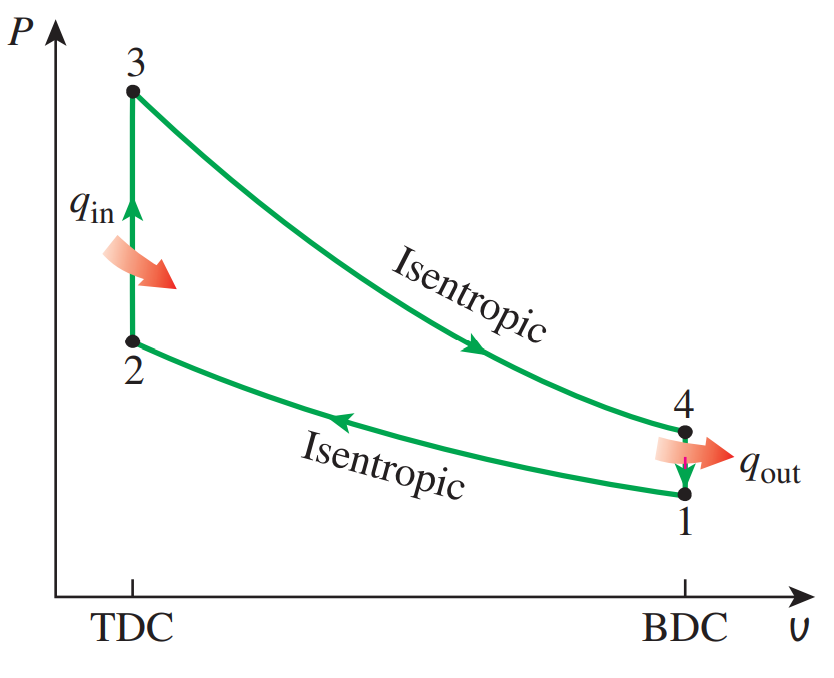
\includegraphics[width=0.4\linewidth]{Images/thermo otto.png}
    \end{center}
    Efficiency for an Otto cycle is given by \[\eta = 1 - \frac{1}{r^{k-1}},\hspace{0.5in}r:=\frac{V_\text{max}}{V_\text{min}},\hspace{0.1in} k:=c_p/c_v\]
    The Otto cycle is limited by \textit{autoignition}, or \textit{engine knock}. For large compression ratios $r$ (around $12$), pockets of fuel-air mixture have a tendency to ignite before the power stroke, causing an effective reduction in volume ratio and reducing efficiency.

    \item[] \textbf{Diesel Cycle}. Diesel engines operate on the Diesel cycle, where air is compressed to high temperatures before pure Diesel fuel is injected and combusted due to the high pressure and high temperature. The Diesel cycle also have four distinct steps:
    \begin{enumerate}
        \item Compression Stroke (replaced by isentropic compression)
        \item Combustion (fuel injection) Stroke (replaced by constant pressure heat addition)
        \item Exhaust Stroke (replaced by isentropic expansion)
        \item Intake Stroke (replaced by constant volume heat rejection)
    \end{enumerate}
    \begin{center}
        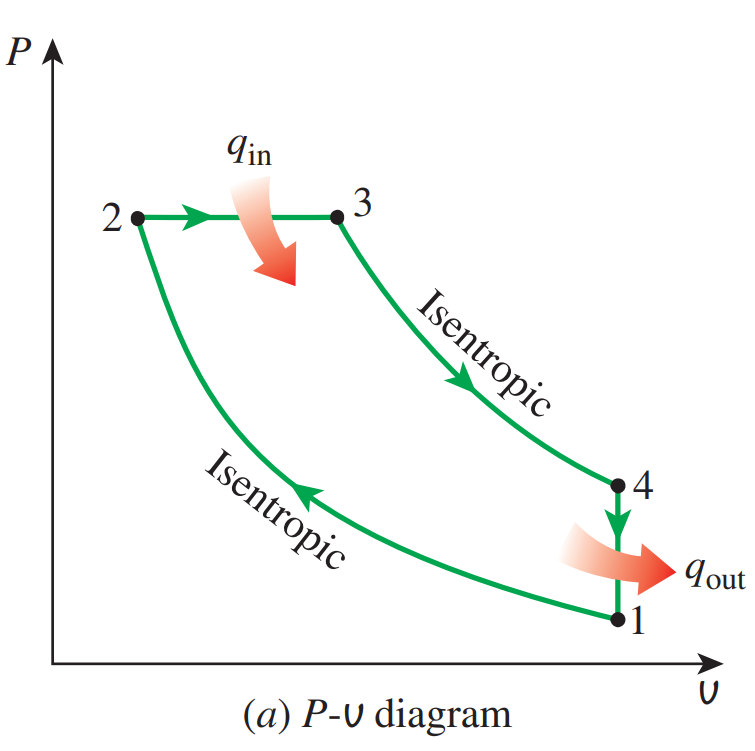
\includegraphics[width=0.4\linewidth]{Images/thermo diesel.png}
    \end{center}
    Efficiency for a Diesel cycle is given by \[\eta = 1-\frac{1}{r^{k-1}}\left[\frac{r_c^k - 1}{k(r_c-1)}\right],\hspace{0.5in}r_c:=\frac{V_3}{V_2}\]
    The Diesel cycle always has a lower efficiency as the same compression ratio, but because combustion is initiated by fuel injection, autoignition is not a concern in Diesel engines and Diesel engines can reach higher raw efficiencies than an engine operating on the Otto cycle.
    \item[] \textbf{Brayton Cycle}. Gas-turbine engines, such as those used in propulsion aircraft, generally operate on a Brayton cycle. A Brayton Cycle uses four devices, and the cycle has four distinct steps:
    \begin{enumerate}
        \item Compressor (isentropic compression)
        \item Heat Exchanger (constant-pressure heat addition)
        \item Turbine (isentropic expansion)
        \item Heat Exchanger (constant-pressure heat rejection)
    \end{enumerate}
    \begin{center}
        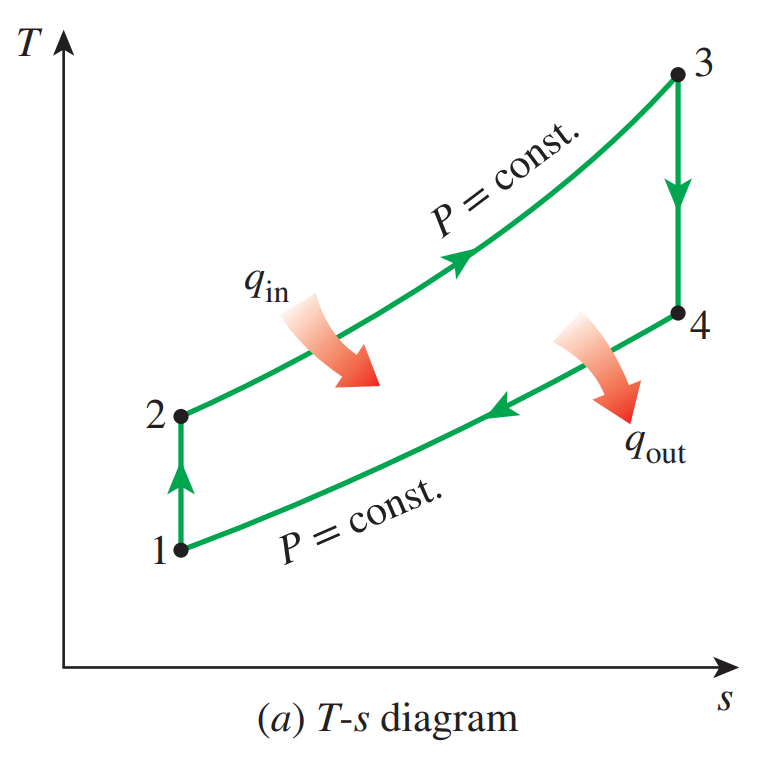
\includegraphics[width=0.4\linewidth]{Images/thermo brayton.png}
    \end{center}
    Efficiency for a Brayton Cycle is given by \[\eta = 1-\frac{1}{r_p^{(k-1)/k}},\hspace{0.5in}r_p=\frac{P_2}{P_1}\] Typical pressure ratios $r_p$ for a Brayton cycle are between $5$ and $20$.
\end{enumerate}

\newpage

Many power plants operate on some form of vapor power cycle, utilizing the phase change of water into steam to produce useful work. The Rankine Cycle is a simple, common cycle utilizing water.

\begin{enumerate}
    \item[] \textbf{Rankine Cycle}. An ideal Rankine cycle utilizes four devices and water in both liquid and vapor form to produce power:
    \begin{enumerate}
        \item Pump (isentropic compression of liquid, initially saturated liquid)
        \item Boiler (constant pressure heat addition to superheated vapor)
        \item Turbine (isentropic expansion)
        \item Condenser (constant-pressure heat rejection)
    \end{enumerate}
    \begin{center}
        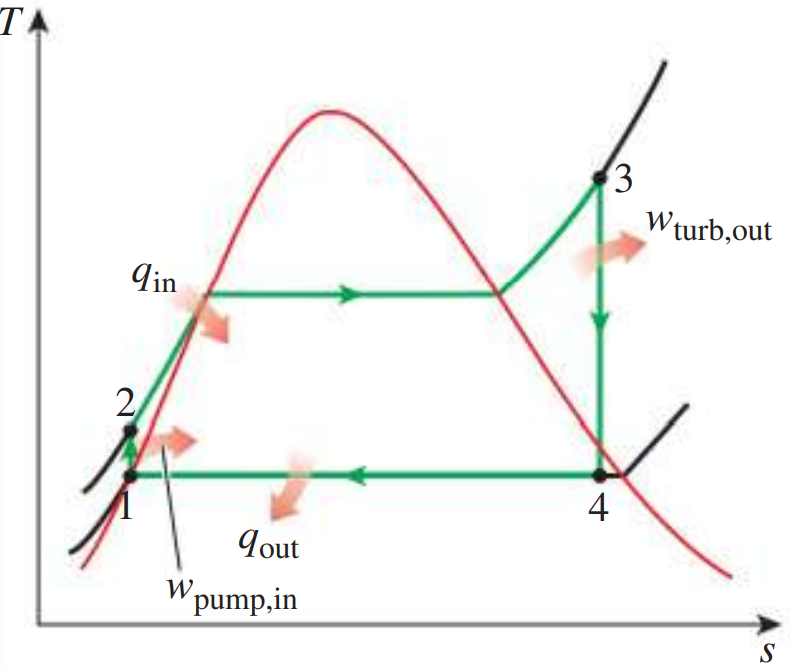
\includegraphics[width=0.4\linewidth]{Images/thermo rankine.png}
    \end{center}
    The efficiency of a Rankine Cycle is given by \[\eta = 1 - \frac{Q_\text{out}}{Q_\text{in}}\] The efficiency of a Rankine cycle may be improved by adding regeneration, diverting some warm water to effectively reduce $Q_\text{in}$.
\end{enumerate}

For power cycles, the \textbf{backwork ratio} is another measure related to efficiency. Backwork ratio is given by \[\text{BWR} = \frac{W_\text{in}}{W_\text{out}}\] Backwork ratio measures what fraction of the output work must be used to power the cycle (in raising the piston, powering the compressor, etc).